\subsection{Expression-first generation and execution}
\label{sec:generator-expression-pipeline}

\citet[Section~2.1]{dascoli2022deep} generate recurrent-sequence examples by
sampling an expression tree, selecting initial conditions, and executing the
recurrence. The implementation adopts this expression-first organization and
retains separate representations of structure and numerical values.
An \emph{abstract syntax tree} (AST) describes the operations and their
arguments; a binding supplies coefficients and positive integer lags. For
example, the skeleton $P_0x_0(t-L_0)+P_1t$ becomes
$0.7x_0(t-2)+0.01t$ after binding its slots. Repeated trajectories preserve
both the tree and its binding while resampling initial conditions or
innovations according to the selected policy.

\begin{figure}[H]
\centering
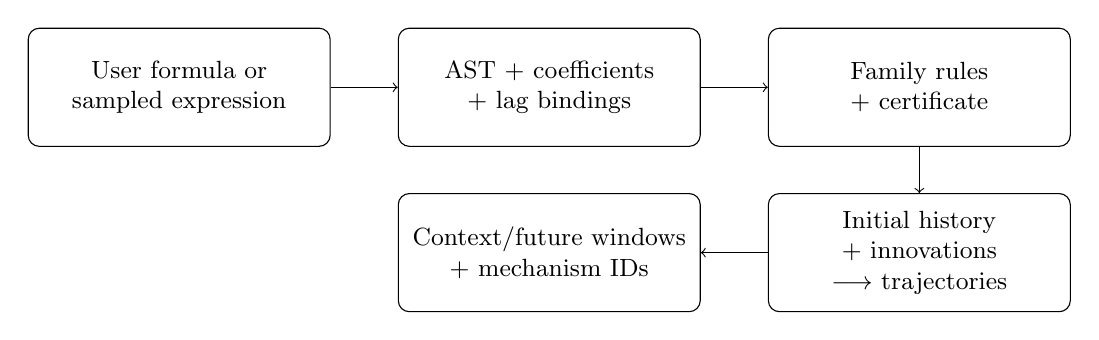
\begin{tikzpicture}[box/.style={draw,rounded corners,align=center,
    text width=3.6cm,minimum height=1.5cm,font=\small}]
\node[box] (tree) at (0,0) {User formula or\\sampled expression};
\node[box] (bound) at (4.7,0) {AST + coefficients\\+ lag bindings};
\node[box] (family) at (9.4,0) {Family rules\\+ certificate};
\node[box] (paths) at (9.4,-2.1) {Initial history\\+ innovations\\$\longrightarrow$ trajectories};
\node[box] (batch) at (4.7,-2.1) {Context/future windows\\+ mechanism IDs};
\draw[->] (tree) -- (bound);
\draw[->] (bound) -- (family);
\draw[->] (family) -- (paths);
\draw[->] (paths) -- (batch);
\end{tikzpicture}
\caption{Implemented generation stages. The selected family determines the
admissible expressions, initialization, and innovation law. The mechanism
record is retained alongside the observations.}
\label{fig:implemented-generator-pipeline}
\end{figure}

\paragraph{Sampling the original trees.}
The base sampler draws a binary-operator count, labels leaves as parameters,
time, or lagged series, and recursively constructs the tree. Its implementation
is in \path{src/tsfmxai/generators/random_expression.py}.
For a subtree containing $o$ binary operators, the
probability of assigning $a$ operators to the left child is proportional to
the number of left shapes times the number of right shapes. These counts
are Catalan numbers. This produces a uniform distribution over ordered full
binary shapes conditional on $o$, before canonicalization. Internal nodes
are labelled addition or multiplication. Zero-operator trees consist of one
leaf; required leaf types must fit the requested size.

The current random base grammar therefore uses binary operations; the
Shao--Wu transformation below adds unary \texttt{Tanh} nodes to the same AST
representation. The wider unary--binary grammar in D'Ascoli et al.
provides the precedent. Our operator probabilities, parameter ranges, forced
lag presence, and multivariate source indices define the project's sampling
prior. Local commutative ordering and slot relabelling provide repeatable
serialization. Algebraic-equivalence experiments separately assess the
stronger objective of assigning one representation to every equivalent
formula.

\paragraph{Executing the retained mechanism.}
At target time $t$, a lag leaf reads $x_{j,t-\ell}$ with $\ell\geq1$.
Equivalently, from the common origin $\tau$, the first generated target uses
$t=\tau+1$. The shared executor
\path{src/tsfmxai/generators/stochastic.py} evaluates every target against the
same previous multivariate history, adds the supplied innovation, and then
appends all new values together. This synchronous update preserves the
intended lag relationships between channels. Model inputs and future targets
can subsequently be separated without changing the recorded equation.

\paragraph{Parallel jobs and repeatability.}
The existing batch builder assigns one mechanism and several trajectories to
each job, then assembles windows with a requested minimum number of distinct
skeletons. It is implemented in
\path{src/tsfmxai/datasets/parallel_batch.py}. Seeds are
derived from the root seed and explicit job, attempt, and stream indices;
ordering is restored when jobs finish. Local random-number generators isolate
these draws from the caller's global random state. Worker-count and seed
independence are tested in the test suite. This batch builder currently uses
the original sampler with acceptance checks; the four-family diagnostic
comparison below evaluates every attempted mechanism and records failures.
